\begin{frame}
	\frametitle{Moltres}
		\begin{itemize}
			\item Moltres is an application code built on the \gls{MOOSE}
			framework, for the simulation of \glspl{MSR}
			\item MOOSE is an open source finite element framework that
			relies on libMesh and PETSc for advanced meshing and PDE
			solver capabilities
			\item Moltres can run transient, fully implicit coupled
			neutronics/thermal-hydraulics simulations of \glspl{MSR}
			\begin{itemize}
				\item Multi-group neutron diffusion (arbitrary groups)
				\item Delayed neutron precursor advection
				\item Incompressible Navier-Stokes for temperature
				advection-diffusion
				\item 2D axisymmetric or 3D modeling
			\end{itemize}
		\end{itemize}
\end{frame}

\begin{frame}
	\frametitle{Moltres}
	\textbf{MSRE (2D axisymmetric model) (Lindsay et al., 2018)}
	\begin{figure}
		\centering
		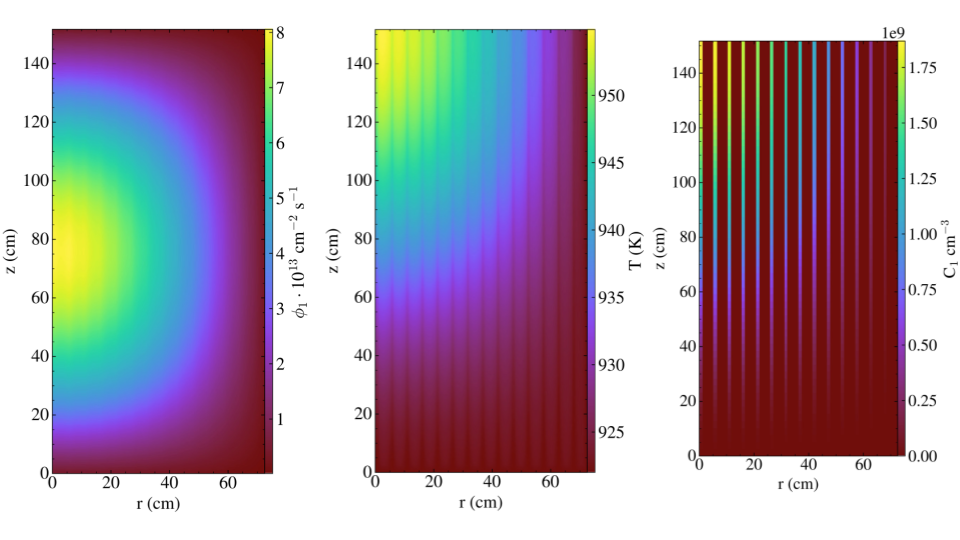
\includegraphics[width=.9\textwidth]{./images/msre}
		\caption{Group 1 flux, temperature, and longest-lived
		precursor distributions of a 2D axisymmetric MSRE model}
	\end{figure}
\end{frame}